\section{Métodos propuestos}\label{sec:propuestas}

Con el objetivo de explorar nuevas estrategias para el entrenamiento de modelos de aprendizaje profundo, \textbf{proponemos dos algoritmos meméticos originales} que, hasta donde sabemos, no han sido previamente estudiados en la literatura. Estos algoritmos combinan un optimizador basado en GD como búsqueda local y una técnica MH utilizada en la literatura para optimización de valores continuos como búsqueda global.

Los algoritmos meméticos han sido seleccionados debido a su \textbf{capacidad para aprovechar las ventajas de la búsqueda global (clave para evitar mínimos locales) y de la búsqueda local}, que incorpora conocimiento específico del problema y permite la convergencia hacia puntos críticos de la función de pérdida \cite{shadeils}. Estas características proporcionan una base teórica sólida para obtener un buen rendimiento en el entrenamiento de modelos.

Las técnicas propuestas, \textbf{SHADE-GD y SHADE-ILS-GD}, se diferencian en la estrategia de búsqueda global empleada: la primera utiliza SHADE como técnica MH, mientras que la segunda emplea SHADE-ILS. Aunque SHADE-ILS ya es un algoritmo memético, pues incorpora una componente de búsqueda local, en nuestra propuesta añadimos una búsqueda local adicional mediante un optimizador basado en GD. Esto se justifica por el conocimiento específico que estos optimizadores tienen sobre el problema, lo que podría mejorar el rendimiento general del algoritmo. Además, esta combinación no ha sido ampliamente explorada en la literatura, y el diseño de algoritmos meméticos ofrece múltiples grados de libertad, lo que puede llevar a resultados interesantes.

La elección de SHADE y SHADE-ILS se basa en que \textbf{ambos pertenecen a la familia de algoritmos DE, la cual ha demostrado ser altamente efectiva en la optimización de parámetros continuos}, como es el caso del entrenamiento de modelos de aprendizaje profundo \cite{shade}. SHADE es un algoritmo bien establecido con un rendimiento sólido en diversos problemas, mientras que SHADE-ILS ha sido específicamente utilizado en la optimización de modelos de aprendizaje profundo, obteniendo buenos resultados en comparación con otras técnicas MH, aunque inferiores a los optimizadores basados en GD \cite{shadeils}. En consecuencia, consideramos que estos algoritmos tienen un alto potencial de mejora mediante su hibridación con técnicas de GD.

Para la búsqueda local basada en GD, seleccionamos el optimizador en función de su rendimiento. Dado que el entrenamiento con optimizadores basados en GD es considerablemente más rápido que con MH, realizamos pruebas con NAG, RMSProp, Adam y AdamW para identificar el más adecuado en cada caso. Este proceso es computacionalmente eficiente y permite adaptar el algoritmo a cada tarea específica. En la mayoría de los experimentos, RMSProp y AdamW han demostrado ser las opciones más competitivas.



Por último, incorporamos el mismo mecanismo de reinicio de población de SHADE-ILS. \textbf{Al final de cada generación, evaluamos la mejora porcentual de la mejor solución respecto a la generación anterior. Si esta mejora es inferior al 5\% durante tres generaciones consecutivas, reiniciamos la población}. En cada reinicio, conservamos la mejor solución, generamos una nueva población y reintroducimos la mejor solución con una pequeña perturbación proveniente de una distribución normal. Mantenemos los valores originales de estos hiperparámetros de SHADE-ILS, aunque realizamos pruebas experimentales con valores cercanos, en las que observamos que sin este mecanismo la población tiende a converger prematuramente y deja de mejorar. Pasamos ahora a describir de forma más pausada el funcionamiento particular de cada propuesta. En la Figura \ref{fig:flowchart} se puede observar el diagrama de flujo que representa el funcionamiento de ambos algoritmos.

\begin{figure}
    \centering
    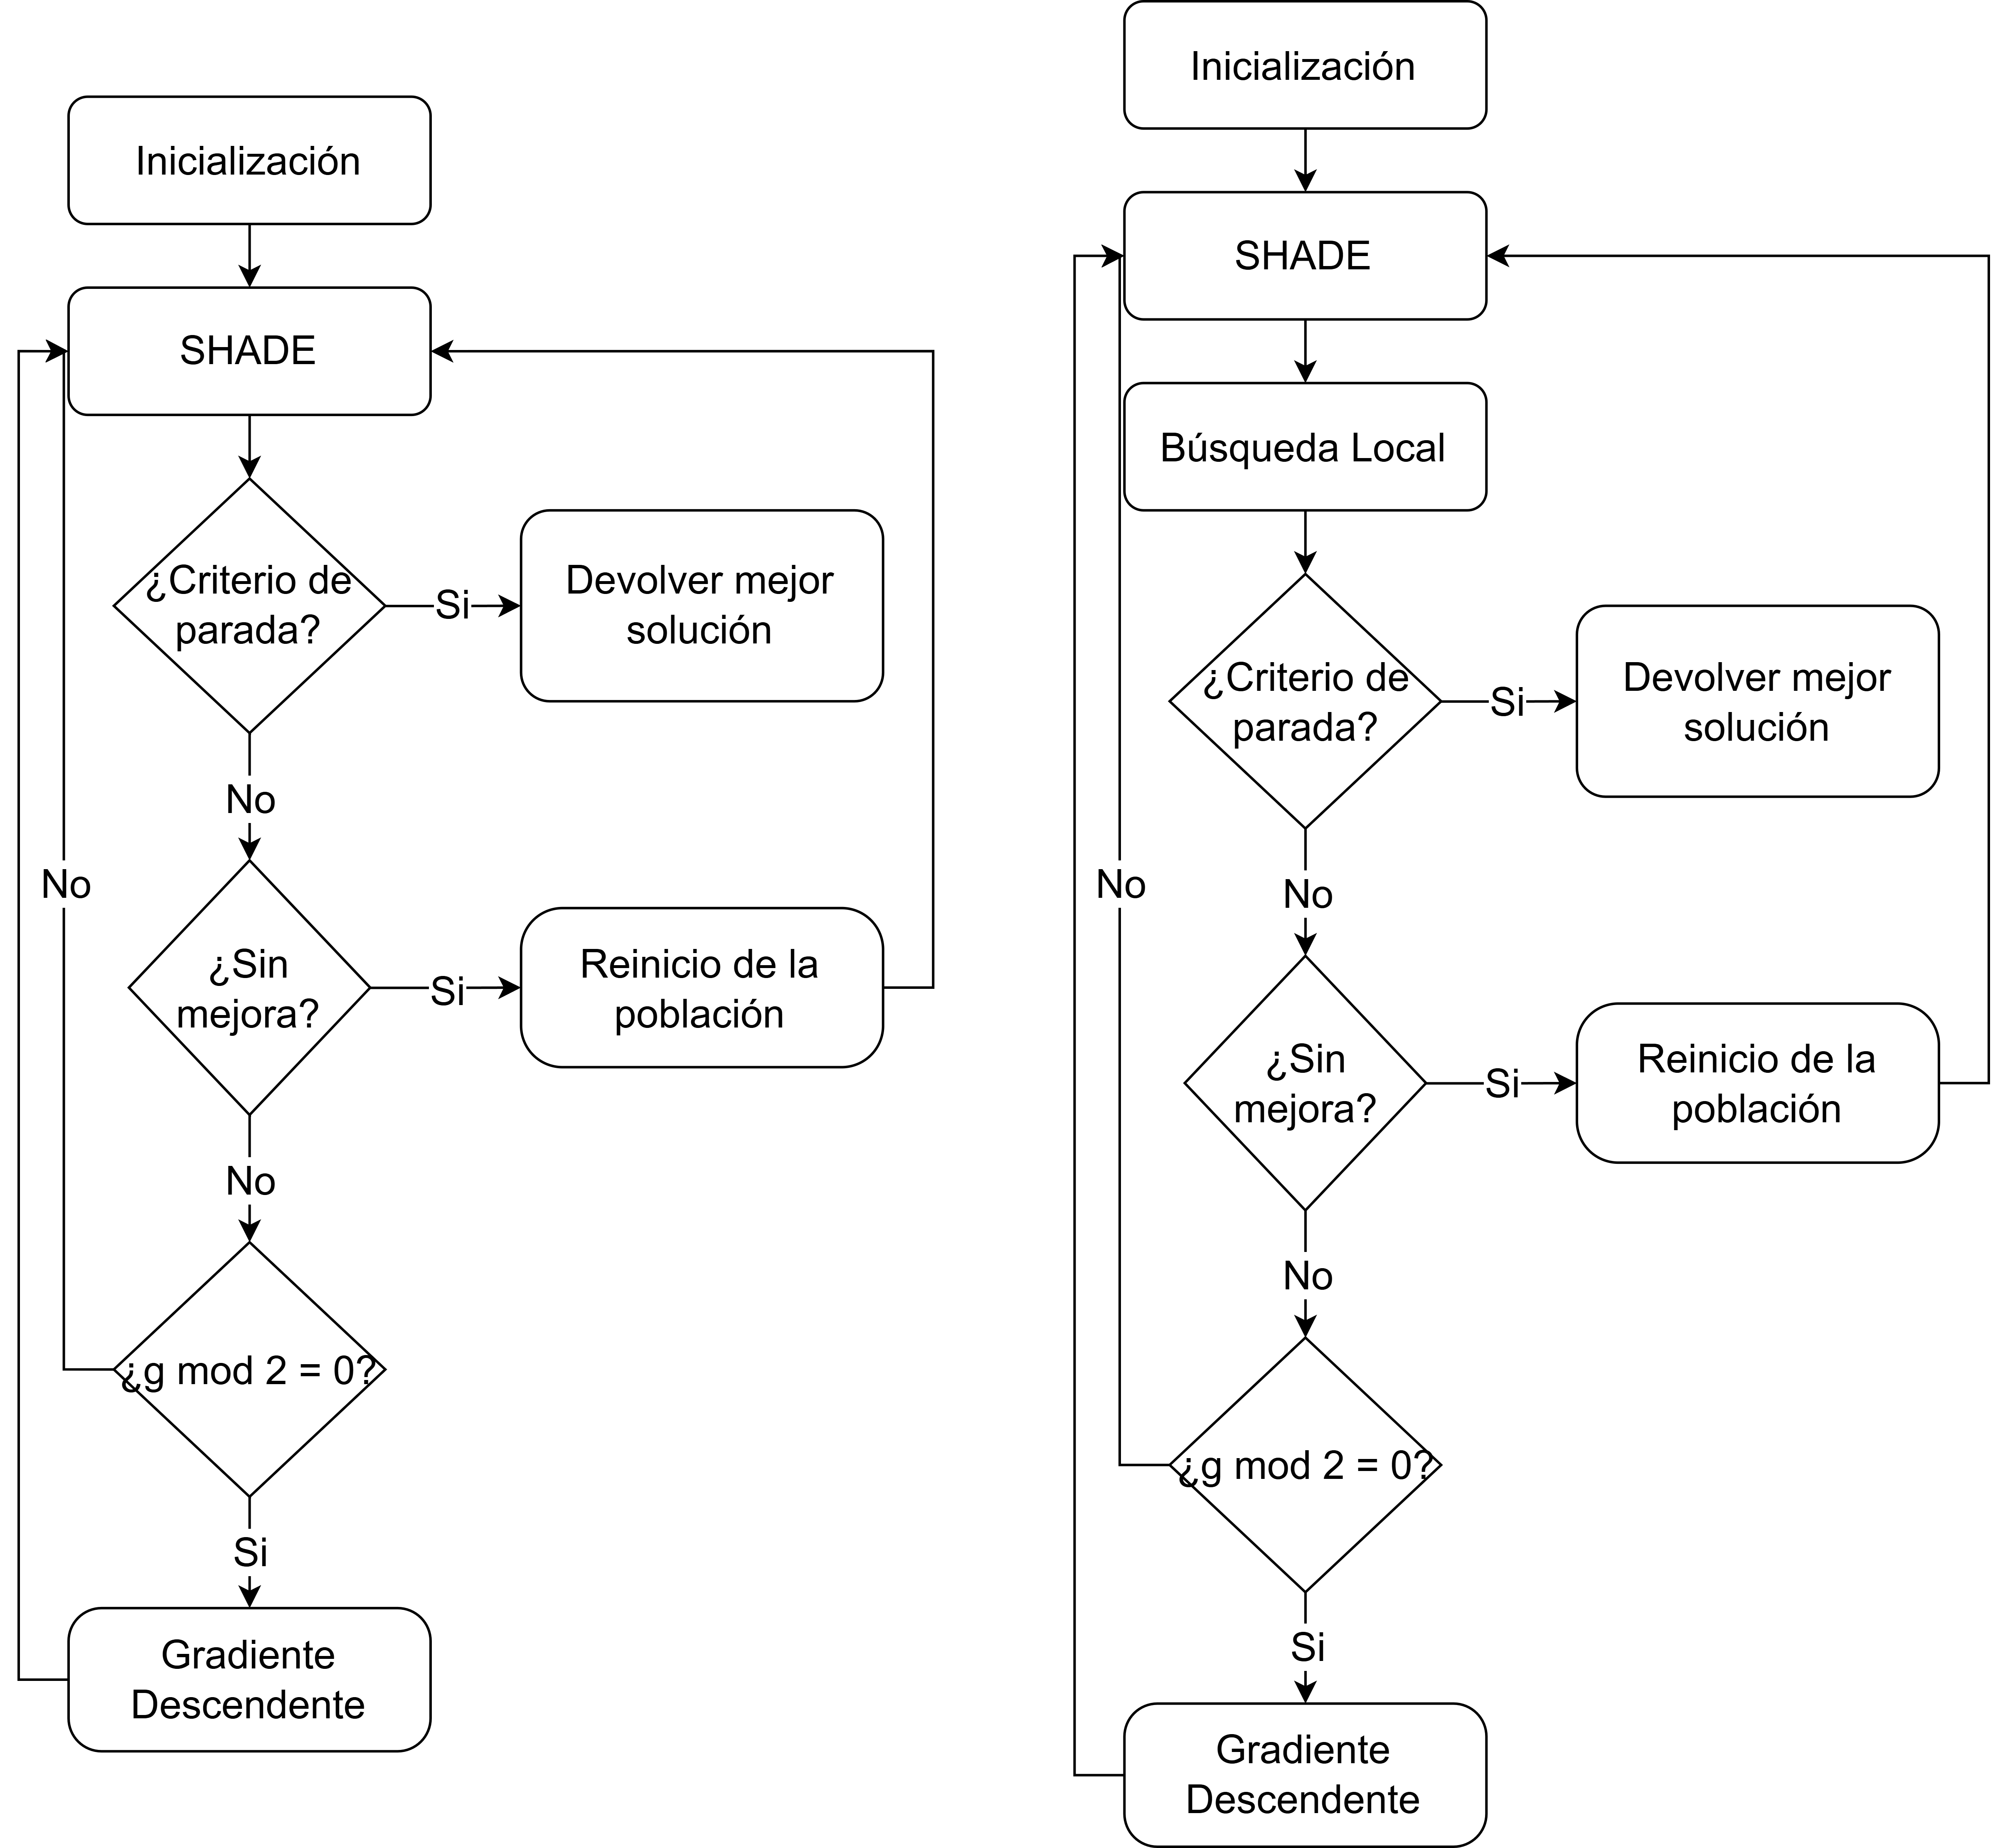
\includegraphics[width=1.0\linewidth]{Plantilla_TFG_latex//imagenes//Inf//Propias/SHADE-GD.png}
    \caption[Diagramas de flujo de los algoritmos SHADE-GD y SHADE-ILS-GD]{La figura muestra la estructura de SHADE-GD (izquierda) y SHADE-ILS-GD (derecha), destacando sus diferencias clave. Ambos algoritmos comienzan con una fase de inicialización en la que se genera una población de soluciones y aplican iterativamente el algoritmo SHADE para actualizar la población mediante operadores evolutivos. SHADE-ILS-GD introduce una etapa adicional de búsqueda local después de cada iteración de SHADE, utilizando L-BFGS-B para refinar la mejor solución encontrada. Luego, ambos algoritmos evalúan un criterio de parada, devolviendo la mejor solución si se cumple. En caso contrario, verifican si ha habido generaciones consecutivas sin mejora significativa y, de ser así, reinician la población conservando la mejor solución con una pequeña perturbación para evitar el estancamiento en óptimos locales. Además, cada dos generaciones, ambos algoritmos aplican descenso de gradiente a un individuo seleccionado aleatoriamente para mejorar la precisión sin comprometer la exploración global. SHADE-ILS-GD se diferencia de SHADE-GD por la inclusión del refinamiento mediante L-BFGS-B en cada iteración y por su estrategia de gestión de la mejor solución global a lo largo del proceso de optimización, lo que mejora la convergencia y reduce el riesgo de estancamiento.}
    \label{fig:flowchart}
\end{figure}

\begin{algorithm}
\caption{Algoritmo SHADE-GD}
\label{alg:shade-gd}
	\begin{algorithmic}
		\State $t := 0$
		\State $g:= 0$
		\State Inicializar Pob$_t$
		\State Inicializar $A$ 
		\State Inicializar $M$ 
		\State Evaluar $x \quad \forall x \in$ Pob$_t$
		\State $m := 0$ 
		
		\While{$t <$ total\_evals}
			\State $i := 0$ 
			\State $g:= g+1$
			\While{$i<$Gen$_{SHADE}$}
				\State $t := t + 1$
				\State $i := i+1$
				\State $f_{\text{prev}} := \text{min} f(x) \quad \forall x \in$ Pob$_{t-1}$
				\State Seleccionar $p$ soluciones para la mutación
				\State Mutar Pob$_{t-1}$ para obtener Pob'
				\State Recombinar Pob' y Pob$_{t-1}$ para obtener Pob''
				\State Evaluar Pob''
				\State Actualizar $A$ y $M$ a partir de Pob'' y Pob$_{t-1}$
				\State Obtener Pob$_t$ a partir de Pob'' y Pob$_{t-1}$
			\EndWhile
			
			\If{$g \text{mod} 2 = 0$}
				\State Seleccionar aleatoriamente $x \in$ Pob$_t$
				\State $x := \text{GD}(x)$
			\EndIf
			
			\State $f_{\text{new}} := \text{min} f(x) \quad \forall x \in$ Pob$_t$
			\If{$\frac{f_{\text{prev}} - f_{\text{new}}}{f_{\text{prev}}} < 0.05$}
				\State $m := m + 1$
			\Else
				\State $m := 0$
			\EndIf
			
			\If{$m \geq 3$}
				\State Reiniciar población conservando la mejor solución con perturbación
				\State $m := 0$
			\EndIf
		\EndWhile
		
		\Return $x_i \in$ Pob$_t : f(x_i) \leq f(x_j) \quad \forall j$
	\end{algorithmic}
\end{algorithm}



\subsection{SHADE-GD}

La propuesta SHADE-GD (Algoritmo \ref{alg:shade-gd}) es una variante del algoritmo SHADE en la que se incorpora un mecanismo de optimización basado en GD para mejorar el refinamiento de las soluciones encontradas. Esta hibridación permite aprovechar la capacidad exploratoria de SHADE y la eficiencia de GD en la explotación local.

\paragraph{1. Inicialización\\}

El algoritmo comienza en $t = 0$ inicializando una población aleatoria de soluciones Pob$_t$, un archivo externo $A$ que almacena soluciones descartadas para mejorar la diversidad, y una memoria $M$ utilizada para adaptar los parámetros de mutación y recombinación. Posteriormente, cada solución de la población es evaluada.  

Además, se definen dos contadores:
\begin{itemize}
    \item $g$: Número de generaciones transcurridas.
    \item $m$: Número de generaciones consecutivas sin mejora significativa.
\end{itemize}

\paragraph{2. Bucle principal de optimización\\}

El proceso de optimización se ejecuta mientras el número total de evaluaciones $t$ no haya alcanzado el límite $\text{total\_evals}$.  

Cada generación en SHADE-GD consiste en un bloque de $\text{Gen}_{SHADE}$ iteraciones SHADE (equivalente a una época de entrenamiento), asegurando que la evolución de la población tenga suficiente estabilidad antes de aplicar la optimización local.  

Para cada iteración dentro de la generación:
\begin{enumerate}
    \item Se actualiza el contador de evaluaciones $t$ y la iteración interna $i$.
    \item Se almacena el mejor valor de la función objetivo en la población anterior, $f_{\text{prev}}$.
    \item Se seleccionan $p$ soluciones para la mutación.
    \item Se genera una población intermedia Pob' mediante mutación y una nueva población Pob'' mediante recombinación.
    \item Se evalúa Pob'' y se actualizan tanto el archivo externo $A$ como la memoria de parámetros $M$.
    \item Se obtiene la nueva población Pob$_t$ seleccionando los mejores individuos entre Pob$_{t-1}$ y Pob''.
\end{enumerate}

\paragraph{3. Aplicación periódica de GD\\}

Cada dos generaciones $(g \mod 2 = 0)$, se selecciona aleatoriamente un individuo de la población y se somete a una optimización local mediante GD. Esta estrategia se justifica experimentalmente, ya que aplicar GD en cada generación conducía a un comportamiento similar al de un optimizador basado exclusivamente en GD, perdiendo la exploración propia de los algoritmos evolutivos.  

Asimismo, la selección aleatoria del individuo evita la concentración de la búsqueda local sobre un único punto, lo que podría inducir sobreajuste y reducir la diversidad de la población.

\paragraph{4. Criterio de reinicio de población\\}

Al finalizar cada generación, se evalúa la mejora relativa de la mejor solución respecto a la generación anterior:

\begin{equation*}
    \Delta f = \frac{f_{\text{prev}} - f_{\text{new}}}{f_{\text{prev}}} \times 100
\end{equation*}

Si la mejora $\Delta f$ es inferior al 5\% durante tres generaciones consecutivas, se activa un mecanismo de reinicio en el que:
\begin{itemize}
    \item Se reconstruye la población aleatoriamente.
    \item Se conserva la mejor solución encontrada hasta el momento.
    \item Se aplica una pequeña perturbación aleatoria a la mejor solución para evitar estancamientos en óptimos locales.
\end{itemize}

Las pruebas experimentales han demostrado que, sin este mecanismo, la población tiende a converger prematuramente y la mejora del algoritmo se detiene.

\paragraph{5. Finalización\\}

El proceso continúa hasta que se alcanzan las total\_evals evaluaciones. Finalmente, se devuelve la mejor solución encontrada en la población final:

\begin{equation*}
    x^* = \arg\min_{x_i \in \text{Pob}_t} f(x_i)
\end{equation*}

Esta solución corresponde al individuo con el menor valor de la función objetivo en la población final.

\paragraph{Conclusión\\}

SHADE-GD mantiene la estructura de SHADE, pero incorpora un refinamiento periódico mediante GD, mejorando la eficiencia de la búsqueda local sin comprometer la capacidad de exploración. Además, el mecanismo de reinicio evita la convergencia prematura y promueve una exploración más efectiva del espacio de soluciones.





\begin{algorithm}
\caption{Algoritmo SHADE-ILS-GD}
\label{alg:shade-ils-gd}
	\begin{algorithmic}
		\State $t := 0$
		\State Inicializar Pob$_t$
		\State $x_0 := (\text{max}_{Pob_t} + \text{min}_{Pob_t})/2$
		\State $x_{\text{best}} := \text{L-BFGS-B}(x_0)$
		\State $x_{\text{global}} := x_{\text{best}}$
		\State $g := 0$ 
		
		\While{t $<$ total\_evals}
			\State $t := t+1$
			\State $f_{\text{prev}} := f(x_{\text{best}})$
			\State $x_{\text{best}}, \text{Pob}_t := \text{SHADE}(\text{Pob}_{t-1})$
			\State $x_{\text{best}} := \text{L-BFGS-B}(x_{\text{best}})$
			
			\If{$t \text{mod} 2 = 0$}
				\State Seleccionar aleatoriamente $x \in$ Pob$_t$
				\State $x := \text{GD}(x)$
			\EndIf
			
			\State $\Delta f := \frac{f_{\text{prev}} - f(x_{\text{best}})}{f_{\text{prev}}} \times 100$
			
			\If{$f(x_{\text{best}}) < f(x_{\text{global}})$}
				\State $x_{\text{global}} := x_{\text{best}}$
			\EndIf
			
			\If{$\Delta f < 5$}
				\State $g := g + 1$
			\Else
				\State $g := 0$
			\EndIf
			
			\If{$g \geq 3$}
				\State Reiniciar población conservando la mejor solución con perturbación
				\State $g := 0$
			\EndIf		
		\EndWhile
		
		\Return $x_{\text{global}}$
	\end{algorithmic}
\end{algorithm}



\subsection{SHADE-ILS-GD}

El algoritmo SHADE-ILS-GD (Algoritmo \ref{alg:shade-ils-gd}) es una extensión híbrida del algoritmo SHADE-ILS que combina tres enfoques de optimización: la exploración global de SHADE, el refinamiento local mediante L-BFGS-B y la optimización periódica con GD. Esta combinación tiene como objetivo mejorar la precisión de las soluciones y evitar la convergencia prematura.

\paragraph{1. Inicialización\\}

El algoritmo comienza en $t = 0$, e inicia los siguientes elementos:

\begin{itemize}
    \item Pob$_t$: Población inicial de soluciones generadas aleatoriamente.
    \item $x_0$: Punto medio del dominio de búsqueda, calculado como $(\text{máximo} + \text{mínimo})/2$.
    \item $x_{\text{best}}$: Mejor solución optimizada localmente mediante el algoritmo L-BFGS-B aplicado a $x_0$. Es la mejor solución encontrada entre dos reinicios de la población.
    \item $x_{\text{global}}$: Mejor solución global encontrada durante la ejecución del algoritmo.
    \item $g$: Contador de generaciones consecutivas sin mejora significativa.
\end{itemize}

\paragraph{2. Bucle principal de optimización}

El algoritmo ejecuta iteraciones hasta que se alcanza el número máximo de evaluaciones $\text{total\_evals}$. Cada iteración realiza las siguientes operaciones:

\begin{enumerate}
    \item Se actualiza el contador de evaluaciones $t$.
    \item Se almacena la mejor solución anterior, $f_{\text{prev}} = f(x_{\text{best}})$.
    \item Se ejecuta una generación completa del algoritmo SHADE sobre la población, obteniendo una nueva población Pob$_t$ y la mejor solución $x_{\text{best}}$.
    \item Se aplica el algoritmo L-BFGS-B a $x_{\text{best}}$ para un refinamiento local un número de $\text{Evals}_{LS}$ iteraciones.
\end{enumerate}

\paragraph{3. Aplicación periódica de GD\\}

Cada dos iteraciones ($t \mod 2 = 0$), se selecciona aleatoriamente un individuo de la población Pob$_t$ y se optimiza localmente utilizando GD. Esta estrategia permite realizar un refinamiento adicional en puntos no explorados por L-BFGS-B y con un método distinto dentro de la misma estrategia, manteniendo la diversidad de soluciones.

\paragraph{4. Actualización de la mejor solución global\\}

En cada iteración, si la mejor solución actual $x_{\text{best}}$ mejora la mejor solución global $x_{\text{global}}$, se actualiza $x_{\text{global}} = x_{\text{best}}$.

\paragraph{5. Criterio de reinicio de población\\}

Se calcula la mejora relativa de la función objetivo como:

\begin{equation*}
    \Delta f = \frac{f_{\text{prev}} - f(x_{\text{best}})}{f_{\text{prev}}} \times 100
\end{equation*}

Si la mejora relativa es inferior al 5\% durante tres generaciones consecutivas, se activa un mecanismo de reinicio que:

\begin{itemize}
    \item Reconstruye la población de manera aleatoria.
    \item Conserva la mejor solución global $x_{\text{global}}$.
    \item Aplica una pequeña perturbación a $x_{\text{global}}$ para escapar de óptimos locales.
\end{itemize}

Este mecanismo previene la convergencia prematura y fomenta una exploración más amplia del espacio de búsqueda.

\paragraph{6. Finalización\\}

El algoritmo concluye cuando se alcanza el límite de evaluaciones $\text{total\_evals}$, devolviendo la mejor solución global encontrada $x_{\text{global}}$:

\begin{equation*}
    x^* = x_{\text{global}}
\end{equation*}

\paragraph{Conclusión\\}

SHADE-ILS-GD combina la exploración global de SHADE con dos técnicas de optimización local: L-BFGS-B para un refinamiento intensivo y GD para mejorar la precisión periódicamente. El mecanismo de reinicio asegura que el algoritmo mantenga la diversidad de soluciones y evita el estancamiento en óptimos locales, lo que lo hace particularmente efectivo para problemas complejos y de alta dimensionalidad.


